\subsection{Sprint 3}

Στην ενότητα αυτή παρουσιάζονται οι τιμές των μετρικών που
χρησιμοποιήθηκαν για κάθε κλάση/enumeration στο τέλος του sprint 3, το
οποίο σημαδεύει και το τέλος της ανάπτυξης του συστήματος. Οι
βασικότερες αλλαγές που πραγματοποιήθηκαν κατά τη διάρκεια του sprint 3
είναι η προσθήκη λειτουργικότητας κόστους και πληρωμών για τις
κρατήσεις, η προσθήκη κλάσεων για τη διαχείριση των τύπων δωματίων
και η αλλαγή του τρόπου παρουσίασης των στοιχείων για τα διαφορετικά
τμήματα λειτουργικότητας της εφαρμογής, όπως η διαχείριση χρηστών,
δωματίων κλπ. Αυτό είχε ως αποτέλεσμα την προσθήκη ακόμα περισσότερων
βοηθητικών κλάσεων διεπαφής αλλά και λίγων κλάσεων με λετουργικότητα
backend.

\subsubsection{Logical Lines Of Code (LLOC)}
\label{section:sprint3LLOC}

Στο σχήμα \ref{fig:sprint3LLOC} εμφανίζεται ο αριθμός των λογικών
γραμμών κώδικα για κάθε κλάση στο τέλος του sprint 3. Παρατηρούμε ότι η
κλάση DBManager είναι εκ νέου αυτή με το μεγαλύτερο μέγεθος, αφού σε
αυτή προστέθηκαν λειτουργίες για τη διαχείριση της βάσης δεδομένων
σχετικές με το κόστος και τις πληρωμές των κρατήσεων αλλά και των τύπων
δωματίων. Το μέγεθος της κλάσης πιθανόν να αρχίζει να γίνεται μη
εύκολα διαχειρίσιμο πια και θα ήταν σίγουρα προτιμότερο να διασπαστεί σε
μικρότερες κλάσεις, η κάθε μία από τις οποίες θα διαχειρίζεται την
επικοινωνία με τη βάση δεδομένων σχετικά μόνο με ένα τύπο δεδομένων.

\begin{figure}
\centering
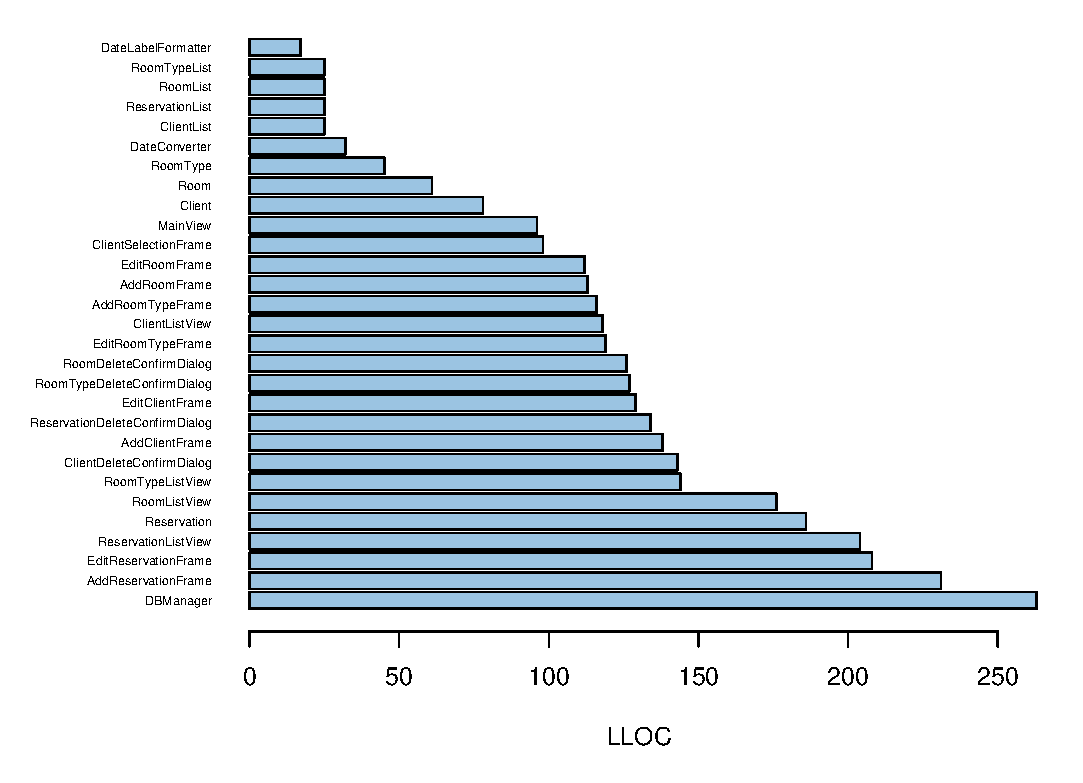
\includegraphics[width=1.0\textwidth]{Sprint3-LLOC-1.eps}
\caption{Λογικές γραμμές κώδικα ανά κλάση στο τέλος του sprint 3}
\label{fig:sprint3LLOC}
\end{figure}

Οι υπόλοιπες κλάσεις με σχετικά μεγάλο μέγεθος είναι οι κλάσεις γραφικής
διασύνδεσης που διαχειρίζονται τις κρατήσεις. Όπως αναφέρθηκε
προηγουμένως στη συζήτηση των τιμών των μετρικών κατά τη διάρκεια του
sprint 2, οι περισσότερες από αυτές θα μπορούσαν πιθανόν να διασπαστούν
σε μικρότερες κλάσεις.

\subsubsection{Clone Coverage (CC)}
\label{section:sprint3CC}

Το σχήμα \ref{fig:sprint3CC} εμφανίζει τις τιμές της μετρικής επανάληψης
κώδικα CC για κάθε κλάση στο τέλος του sprint 3. Όπως και στο αντίστοιχο
σχήμα για το sprint 2, και σε αυτή την περίπτωση οι κλάσεις με τις
μεγαλύτερες τιμές είναι με διαφορά οι κλάσεις γραφικής διασύνδεσης. Όπως
και στα αντίστοιχα αποτελέσματα του sprint 2, η επανάληψη κώδικα σε
αυτές τις κλάσεις οφείλεται κυρίως στον κώδικα που έχει παραχθεί
αυτόματα με το σχεδιασμό και την τοποθέτηση των διάφορων γραφικών
συστατικών όπως κουμπιά, λίστες κλπ στα αντίστοιχα παράθυρα.

\begin{figure}
\centering
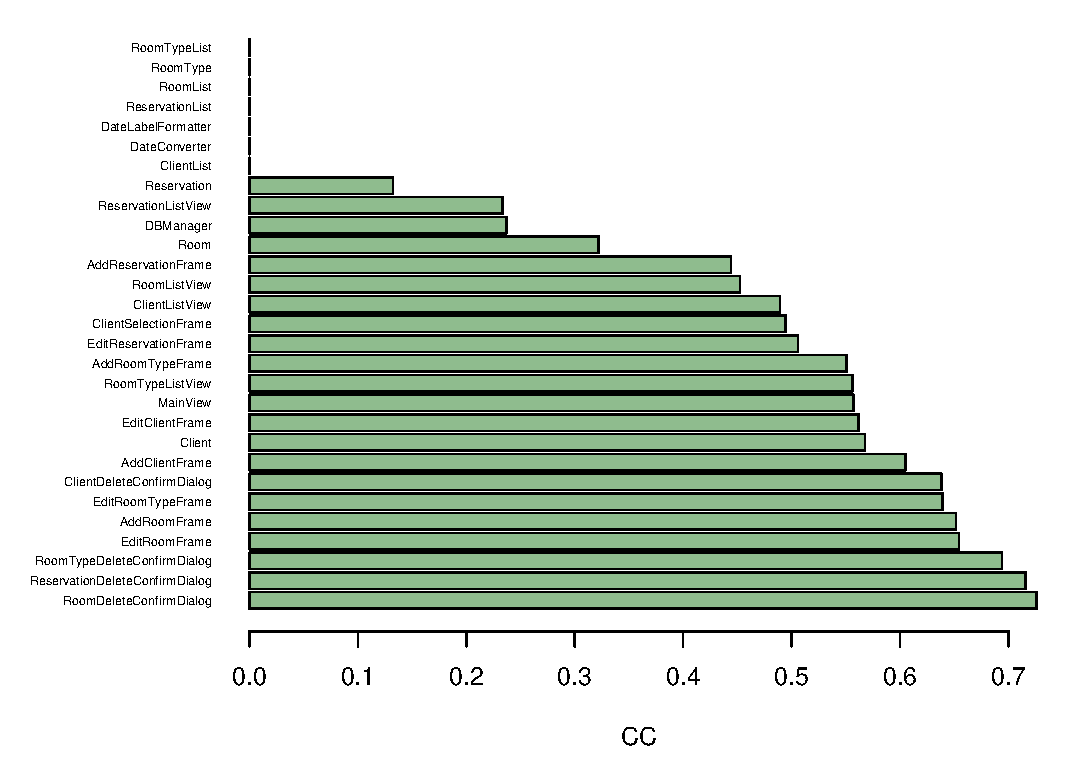
\includegraphics[width=1.0\textwidth]{Sprint3-CC-1.eps}
\caption{Τιμές της μετρικής CC ανά κλάση στο τέλος του sprint 3}
\label{fig:sprint3CC}
\end{figure}

Για τις κλάσεις backend με υψηλές τιμές, όπως η κλάση Client ισχύουν τα
όσα ειπώθηκαν στην ενότητα \ref{section:sprint1CC}, με την
επαναληψιμότητα να οφείλεται σε κώδικα ελέγχου της μεθόδου main και ο
οποίος ουσιαστικά δεν επηρεάζει την λειτουργία του συστήματος στο
παραμικρό.

\subsubsection{McCabe’s Cyclomatic Complexity (McCC)}
\label{section:sprint3McCC}

Στο σχήμα \ref{fig:sprint3McCC} εμφανίζονται οι τιμές της μετρικής
κυκλωματικής πολυπλοκότητας McCC για κάθε κλάση στο τέλος του sprint 3.
Οι κλάσεις οντοτήτων που παρουσιάζουν τις υψηλότερες τιμές είναι οι
Reservation και DBManager.

\begin{figure}
\centering
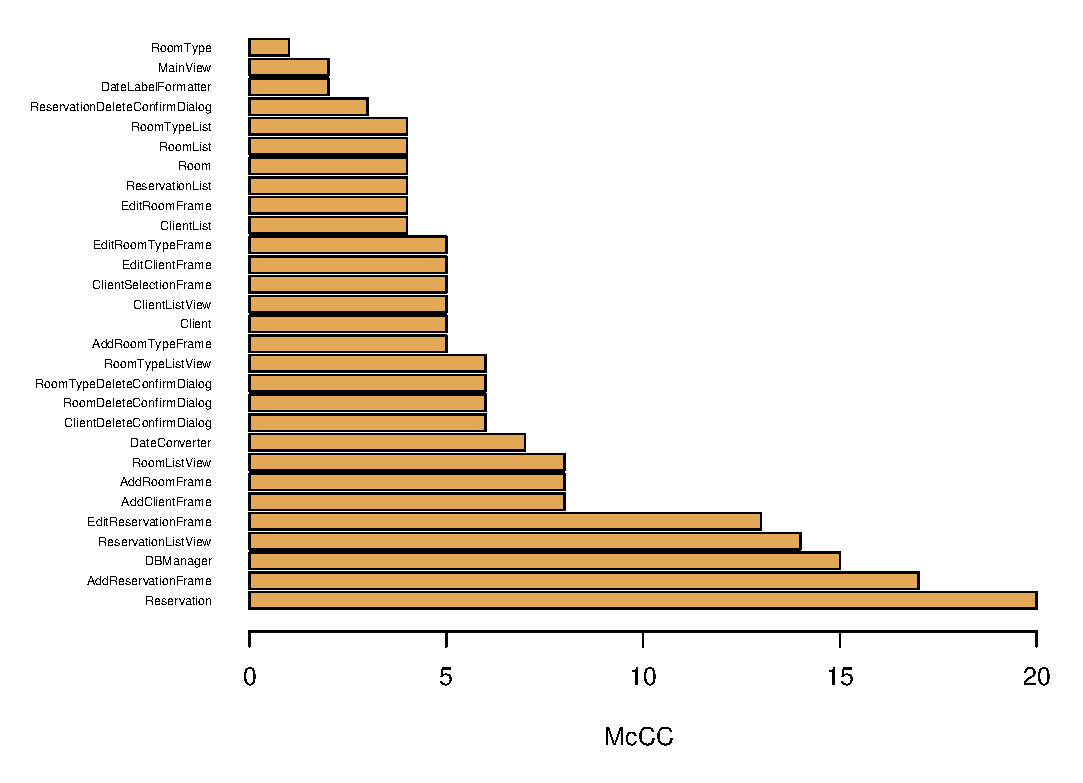
\includegraphics[width=1.0\textwidth]{Sprint3-McCC-1.eps}
\caption{Τιμές της μετρικής κυκλωματικής πολυπλοκότητας McCC ανά κλάση στο τέλος του sprint 3}
\label{fig:sprint3McCC}
\end{figure}

Εξετάζοντας τον κώδικα της κλάσης Reservation, διαπιστώθηκε ότι αρκετές
από τις δομές ελέγχου που χρησιμοποιούνται, περίπου οι μισές από τις
συνολικές, βρίσκονται στη μέθοδο main,
η οποία χρησιμοποιείται για τον έλεγχο της σωστής λειτουργικότητας της
κλάσης. Ο κώδικας αυτός μπορεί να αφαιρεθεί στο σύνολό του από την
κλάση χωρίς να επηρεαστεί στο παραμικρό η λειτουργικότητα του
συστήματος. Έτσι η υψηλή τιμή για την κλάση Reservation είναι μέχρι ενός
σημείου πλασματική. Σε οποιαδήποτε περίπτωση, οι έλεγχοι που έχουν
προστεθεί πρόχειρα στη μέθοδο main της κλάσης θα μπορούσαν να
μεταφερθούν σε νέα unit testing κλάση.

Κατά τη διάρκεια του sprint 3 προστέθηκε κώδικας στην κλάση Reservation
σχετικός με τη διαχείριση του κόστους των κρατήσεων και των αντίστοιχων
πληρωμών από τους πελάτες. Θα μπορούσε αυτός ο κώδικας να διαχωριστεί σε
μια νέα κλάση, οπότε η τιμή της μετρικής θα μειωνόταν ακόμα περισσότερο.

Όπως αναφέρθηκε προηγουμένως, η κλάση DBManager πιθανόν αρχίζει να
γίνεται μη εύκολα διαχειρίσιμη και ενδεχομένως περαιτέρω ανάπτυξη του
συστήματος να παρουσίαζε δυσχέρεια στη συντήρησή του. Το πρόβλημα μπορεί
να λυθεί με τη διάσπαση της κλάσης σε μικρότερες όπως έχει ήδη
περιγραφεί.

Για τις κλάσεις γραφικής διασύνδεσης με υψηλές τιμές της μετρικής, οι
οποίες είναι για ακόμα μία φορά οι κλάσεις που σχετίζονται με τη
διαχείριση των κρατήσεων. Το πρόβλημα προέρχεται από τον κώδικα που
περιλαμβάνουν για τον έλεγχο εγκυρότητας και διαθεσιμότητας των
κρατήσεων, ο οποίος θα μπορούσε να διαχωριστεί σε μια νέα κλάση η οποία
θα υλοποιεί μόνο αυτή τη λειτουργικότητα.

Οι τιμές της κυκλωματικής πολυπλοκότητας για τις υπόλοιπες κλάσεις του
συστήματος χαρακτηρίζονται ως ικανοποιητικές, χωρίς να θεωρούνται
απαραίτητες αναδομήσεις για τη βελτίωσή τους.

\subsubsection{Lack of Cohesion in Methods 5 (LCOM5)}
\label{section:sprint3LCOM5}

Το σχήμα \ref{fig:sprint3LCOM5} δείχνει τις τιμές της μετρικής έλλειψης
συνεκτικότητα LCOM5 για κάθε κλάση στο τέλος του sprint 3. Παρατηρούμε
ότι η κλάση με την υψηλότερη τιμή είναι η RoomType, κλάση η οποία
προστέθηκε κατά τη διάρκεια του sprint 3. Αν και η τιμή της μετρικής
LCOM5 είναι ανησυχητική από μόνη της, το μικρό μέγεθος της κλάσης, το
οποίο είναι μικρότερο από 50 γραμμές κώδικα (σχ.\ \ref{fig:sprint3LLOC}),
οδηγεί στο συμπέρασμα ότι δεν είναι απαραίτητη
κάποια αναδόμηση για τη βελτίωση της μετρικής.

\begin{figure}
\centering
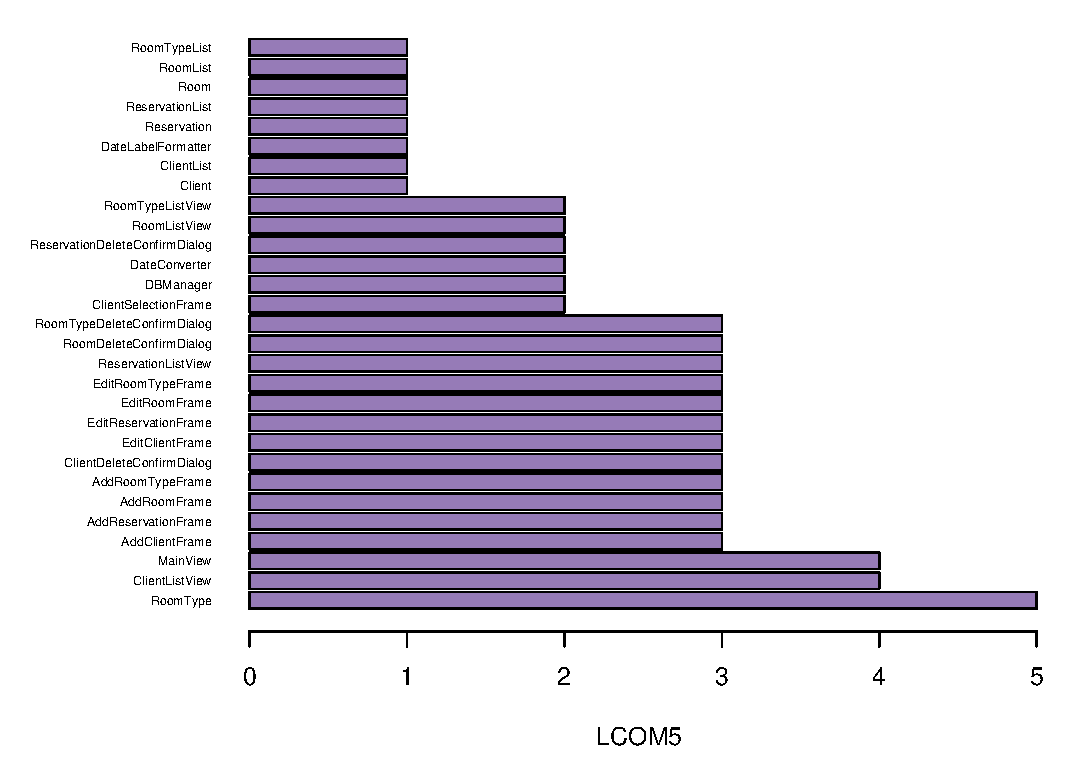
\includegraphics[width=1.0\textwidth]{Sprint3-LCOM5-1.eps}
\caption{Τιμές της μετρικής έλλειψης συνεκτικότητας LCOM5 ανά κλάση στο τέλος του sprint 3}
\label{fig:sprint3LCOM5}
\end{figure}

Αντίστοιχα μικρές είναι και οι κλάσεις γραφικής διασύνδεσης MainView και
ClientListView που ακολουθούν, λαμβάνοντας υπόψη το μέγεθος του κώδικα
που έχει παραχθεί αυτόματα για τα γραφικά συστατικά των αντίστοιχων
παραθύρων. Το ίδιο ισχύει και για τις επόμενες στη σειρά κλάσεις οι
οποίες παρουσιάζουν τιμή της μετρικής ίση με 3. Στο σύνολό τους
πρόκειται για κλάσεις γραφικής διασύνδεσης μικρού μεγέθους. Εξαίρεση
αποτελούν οι κλάσεις διαχείρισης των κρατήσεων AddReservationFrame και
EditReservationFrame. Γι' αυτές, όπως έχει αναφερθεί προηγουμένως, θα
ήταν πιθανόν προτιμότερο να διαχωριζόταν ο κώδικας ελέγχου εγκυρότητας
και διαθεσιμότητας των κρατήσεων σε νέες κλάσεις.

\subsubsection{Coupling Between Object classes (CBO)}
\label{section:sprint3CBO}

\begin{figure}
\centering
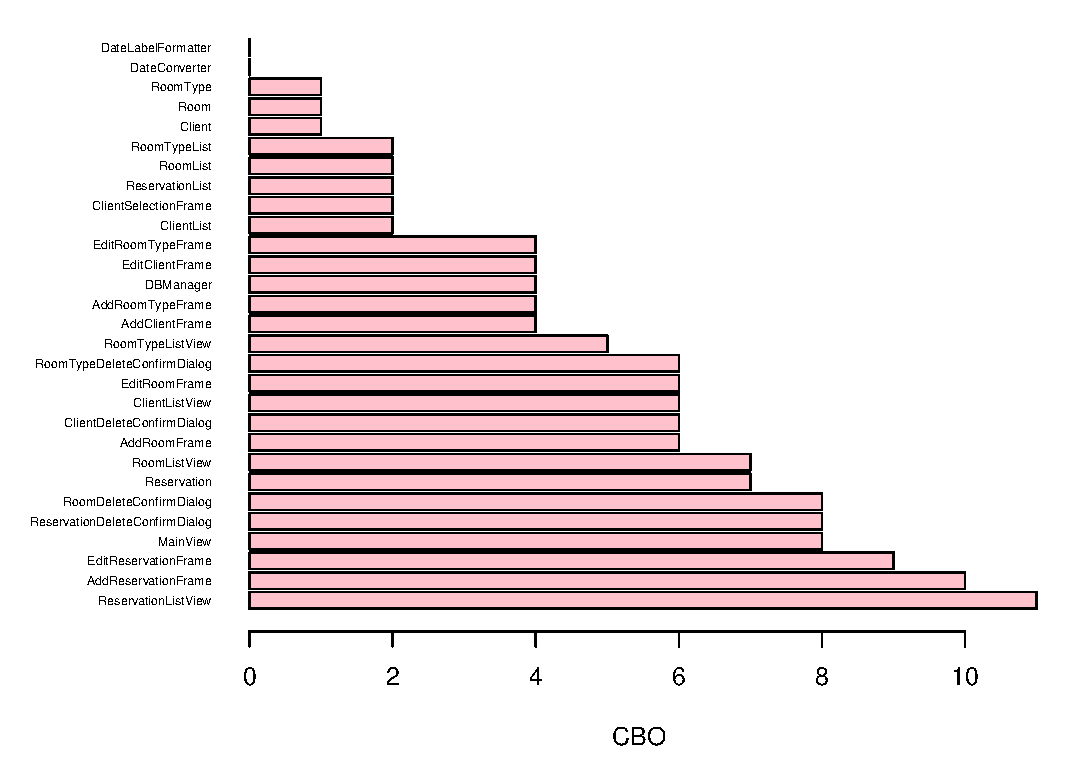
\includegraphics[width=1.0\textwidth]{Sprint3-CBO-1.eps}
\caption{Τιμές της μετρικής σύζευξης CBO ανά κλάση στο τέλος του sprint 3}
\label{fig:sprint3CBO}
\end{figure}
